\documentclass[final]{beamer}

% ====================
% Packages
% ====================

\usepackage[T1]{fontenc}
\usepackage{lmodern}
\usepackage[size=custom,width=120,height=72,scale=1.0]{beamerposter}
\usetheme{gemini}
\usecolortheme{JHU}
\usepackage{graphicx}
\usepackage{booktabs}
\usepackage{tikz}
\usepackage{pgfplots}
\usepackage{graphbox}

\pgfplotsset{compat=1.17}
\usepackage[belowskip=-15pt,aboveskip=8pt]{caption}

% ====================
% Lengths
% ====================

% If you have N columns, choose \sepwidth and \colwidth such that
% (N+1)*\sepwidth + N*\colwidth = \paperwidth
\newlength{\sepwidth}
\newlength{\colwidth}
\setlength{\sepwidth}{0.000\paperwidth}
\setlength{\colwidth}{0.235\paperwidth}

\newcommand{\separatorcolumn}{\begin{column}{\sepwidth}\end{column}}

% ====================
% Title
% ====================

\title{Haplotype-aware inference of human chromosome abnormalities}

\author{Daniel Ariad \inst{1} \and Stephanie M. Yan \inst{1} \and Manuel Viotti \inst{2} \and Andrea R. Victor \inst{2} \and Rajiv C. McCoy \inst{1}}

\institute[shortinst]{\inst{1} Johns Hopkins University | Krieger School of Arts \& Sciences | Baltimore, MD \samelineand \inst{2} Zouves Fertility Center | Foster City, CA}

% ====================
% Footer (optional)
% ====================

\footercontent{
\href{mailto:daniel@ariad.org}{daniel@ariad.org}
   \hfill
  \href{https://mccoy-lab.org/}{
McCoy Lab – Human Genomics @ JHU} \hfill
  \href{mailto:rajivmccoy@jhu.edu}{rajiv.mccoy@jhu.edu}}
  
% (can be left out to remove footer)

% ====================
% Logo (optional)
% ====================

% use this to include logos on the left and/or right side of the header:
% \logoright{\includegraphics[height=7cm]{logo1.pdf}}
% \logoleft{\includegraphics[height=7cm]{logo2.pdf}}

% ====================
% Body
% ====================

\begin{document}
\addtobeamertemplate{headline}{}
{
    \begin{tikzpicture}[remember picture,overlay]
      \node [anchor=north west, inner sep=3cm] at ([xshift=0.0cm,yshift=2.5cm]current page.north west)
      {
\includegraphics[height=7.0cm]{logos/university.logo.large.horizontal.white.eps}}; % also try shield-white.eps
      \node [anchor=north east, inner sep=3cm] at ([xshift=0.0cm,yshift=2.5cm]current page.north east)
      {
\includegraphics[height=8.0cm]{logos/krieger.logo.large.horizontal.white.eps}};
    \end{tikzpicture}
}

\begin{frame}[t]
\begin{columns}[t]
\separatorcolumn

\begin{column}{\colwidth}

  \begin{block}{Introduction}
%\heading{Motivation}

    \begin{figure}
      \centering
     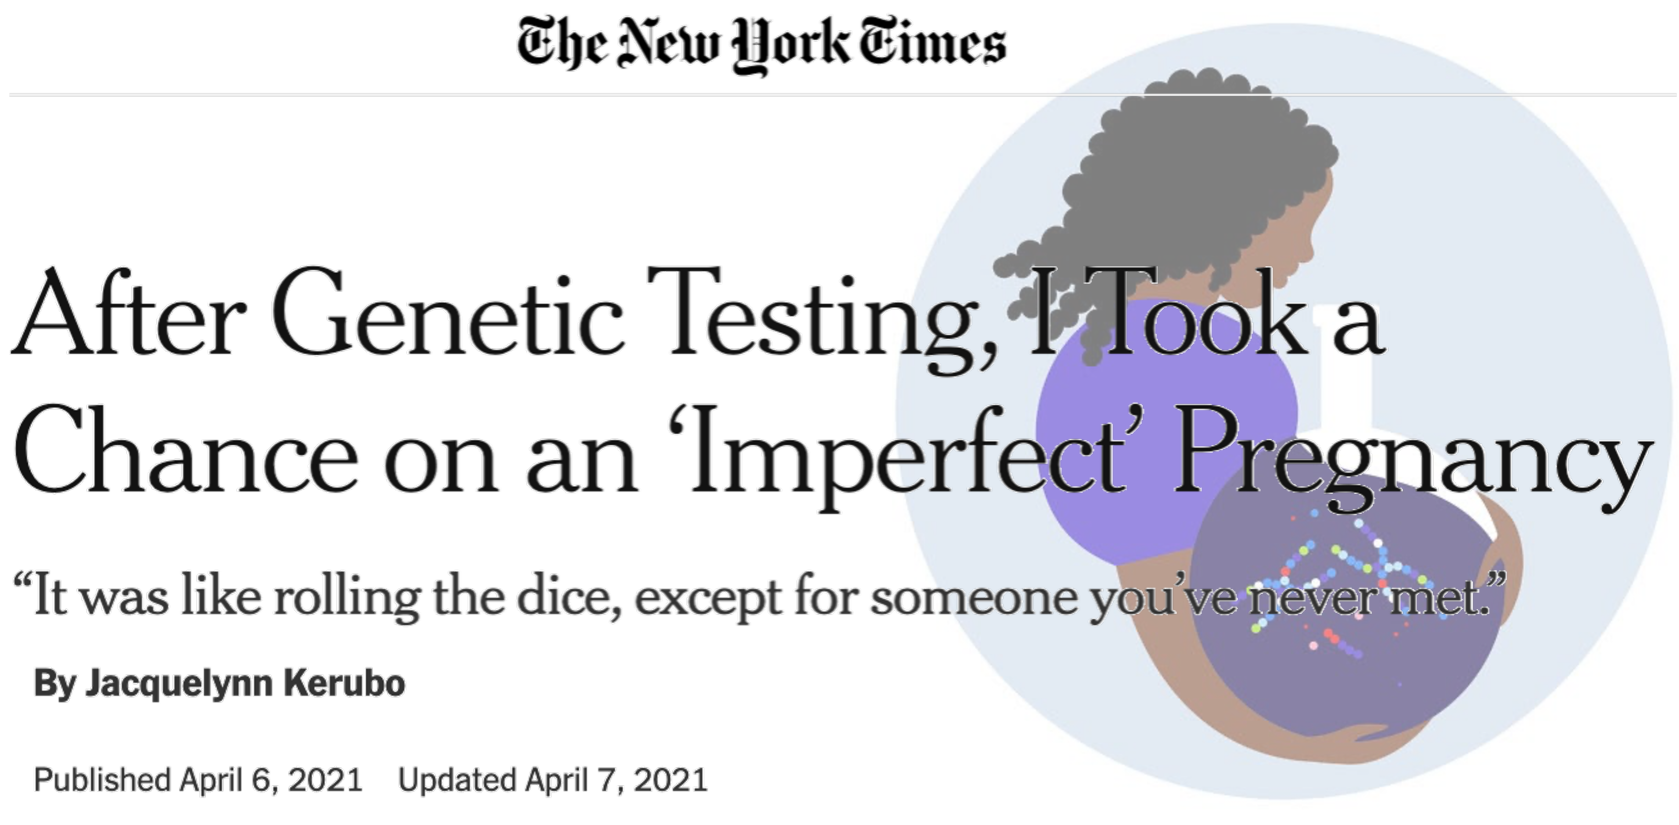
\includegraphics[width=0.45\linewidth,align=c]{figures/new_york.pdf}\hspace{1cm}
     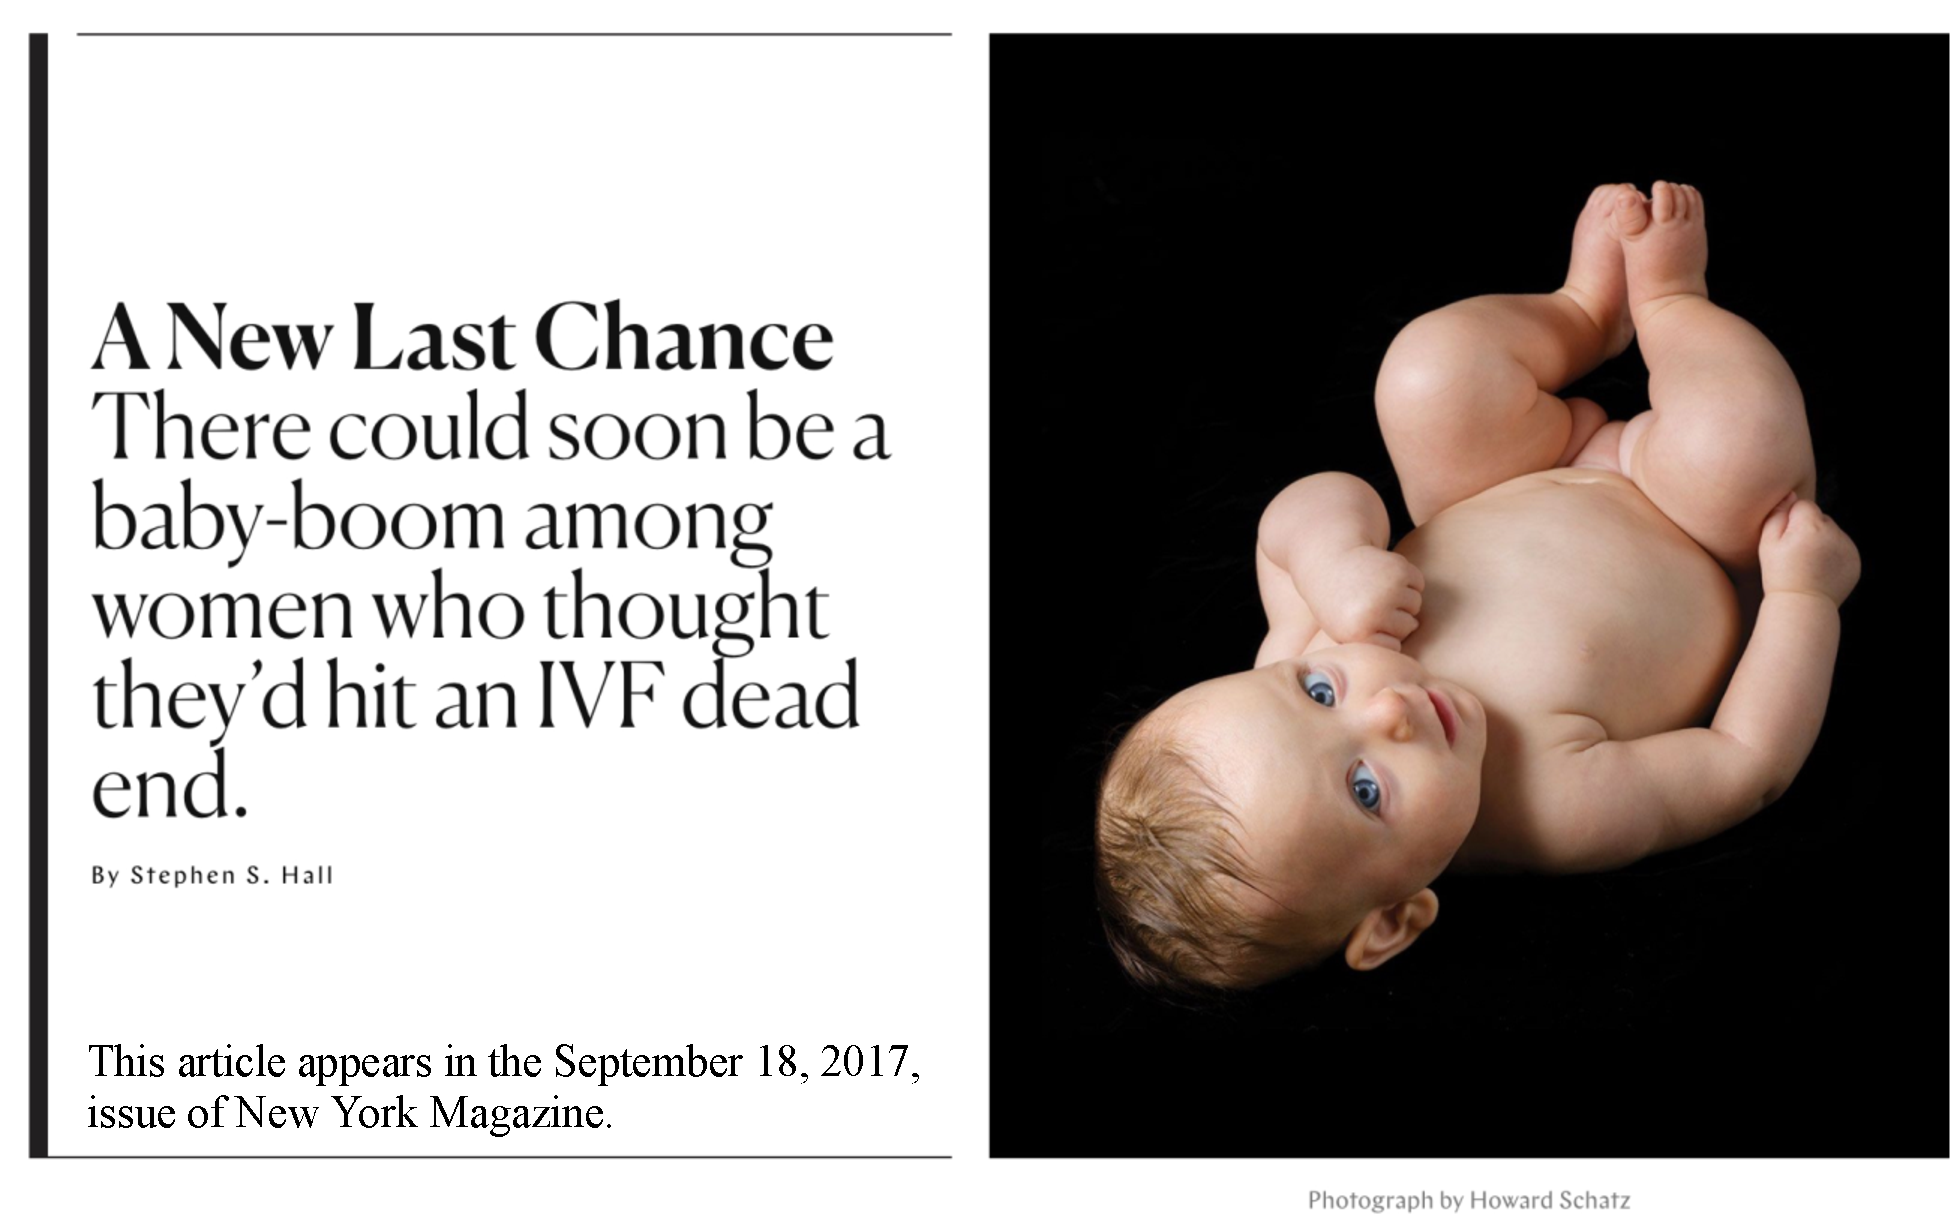
\includegraphics[width=0.45\linewidth,align=c]{figures/nymag.pdf}

      \caption{Mosaic (i.e., mitotic) aneuploidy may be compatible with healthy birth.}
    \end{figure}
    
\begin{itemize}
     \item Preimplantation genetic testing for aneuploidy (PGT-A) has been devised as an approach to improve IVF outcomes by prioritizing chromosomally normal (i.e. euploid) embryos for transfer based on genetic analysis of embryo biopsies.
     
\item Extra or missing chromosomes (aneuploidy) is the leading cause of human pregnancy loss and congenital disorders. 

\item While meiotic aneuploidies are unambiguously harmful, mitotic errors, which generate mosaic embryos possessing both normal and aneuploid cells, are common and potentially compatible with healthy live birth. 

\item The ability to distinguish meiotic- and mitotic-origin aneuploidies during PGT-A may thus prove valuable for enhancing IVF outcomes.
\end{itemize}

%\heading{Aspects of maternal age and procedure in IVF }
    \begin{figure}
      \centering
           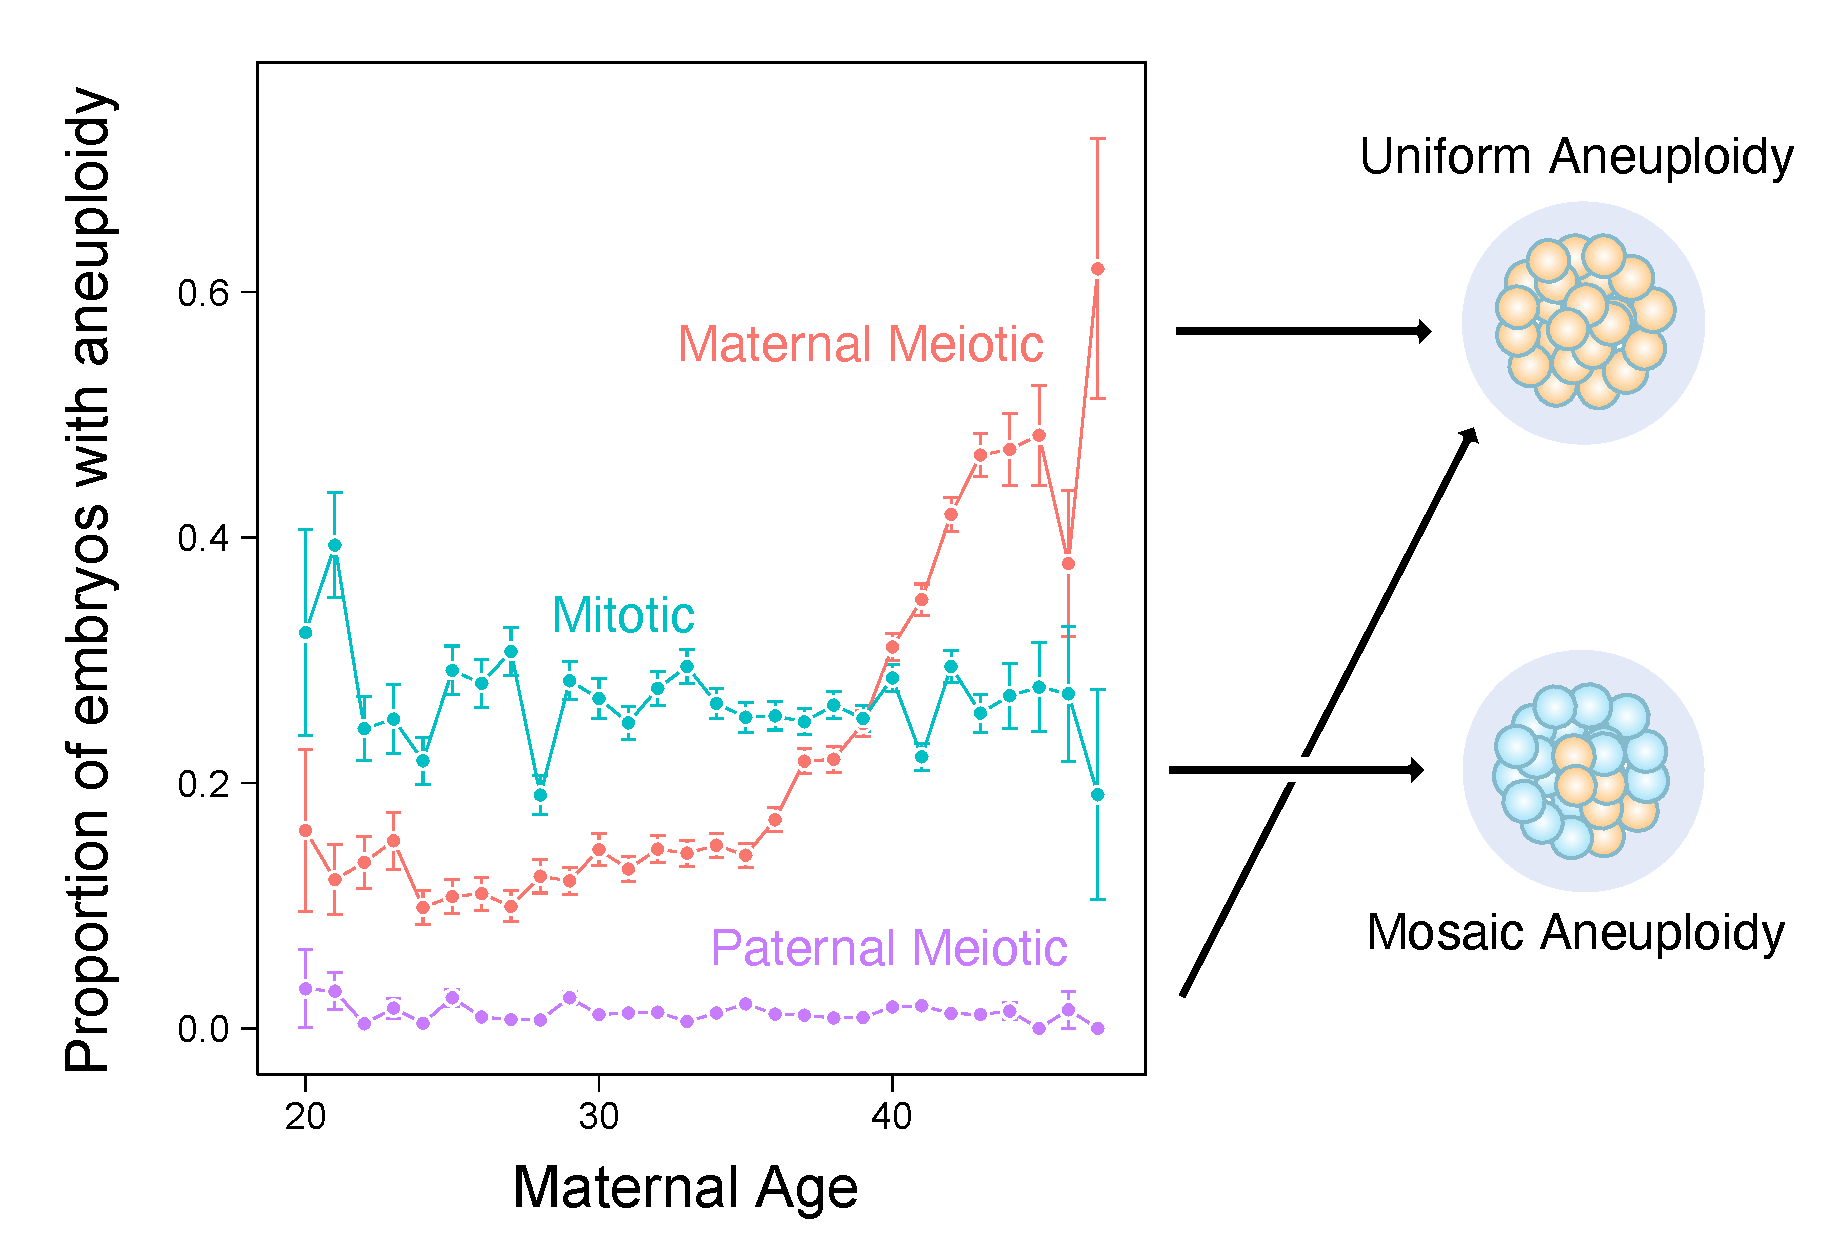
\includegraphics[width=0.59\linewidth,align=c]{figures/BPH_and_SPH_errors_vs_maternal_age.pdf}
           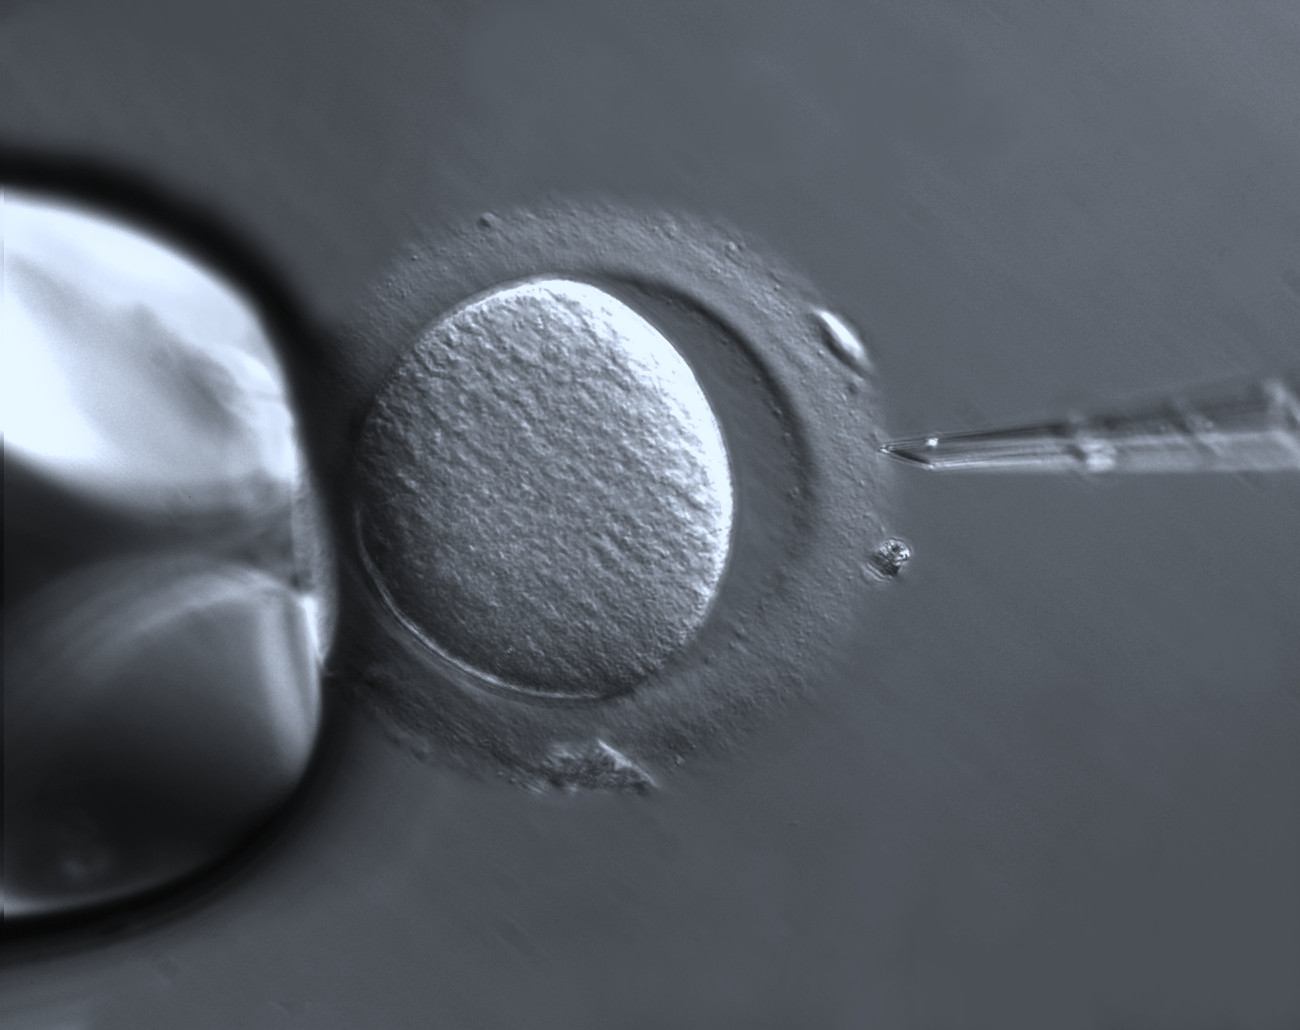
\includegraphics[width=0.4\linewidth,align=c]{figures/Oocyte_with_Zona_pellucida_(27771482282)_original.jpg}

      \caption{Meiotic and mitotic errors contribute to human aneuploidy}
    \end{figure}
    \begin{itemize}
 
      %  \item First introduced in the 1990s, PGT-A has been the subject of long-standing controversy in the IVF field, with some meta-analyses and clinical trials drawing its purported benefits into question.  

       \item Aneuploidies of maternal meiotic origin increase in frequency with age.
    %    \item Aneuploidies of paternal meiotic origin are comparatively rare and constant with age.
        \item Aneuploidies of mitotic origin are prevalent and constant across all ages. 
    %    \item Meiotic errors produce uniformly aneuploid embryos, while %mitotic errors generate chromosomal mosaicism.
    %    This situation occurs in $~15\%$ of all IVF cycles for patients %$\leq35$ years old, but rapidly increases to $>60\%$ of IVF cycles for %patients in their mid 40’s.
     \item The current PGT-A comprise low-coverage whole-genome sequencing of DNA extracted from 5-10 trophoblast cells of day-5 embryos.
    %    \item The ability to classify meiotic and mitotic aneuploidies holds %promise for recovering viable embryos from the many IVF cycles where zero %euploid-testing embryos are produced.
    \end{itemize}
    

  \end{block}

  \begin{alertblock}{Motivation}

    \begin{itemize}
     \item To date, few methods have explicitly attempted to distinguish the patterns of transmission of individual parental homologous chromosomes, which may inform the classification of meiotic and mitotic aneuploidies. 
    \item The few exceptions require genomic data from parents, as well as embryos, and/or are not designed for low-coverage sequencing data— the current standard for PGT-A.
    \item Distinguishing viable forms of mosaic aneuploidy from harmful meiotic aneuploidy could recover healthy embryos from IVF cycles otherwise deemed unsuccessful.
    \end{itemize}  
    
    \end{alertblock}

\end{column}

\separatorcolumn

\begin{column}{\colwidth}

\begin{block}{Signatures of meiotic and mitotic trisomy}
Notably, trisomies of meiotic origin are expected to produce a genetic signature characterized by the presence of three unique parental haplotypes (two from a single parent) and distinct from the mitotic trisomy signature of only two unique haplotypes chromosome-wide.
    \begin{figure}
      \centering
     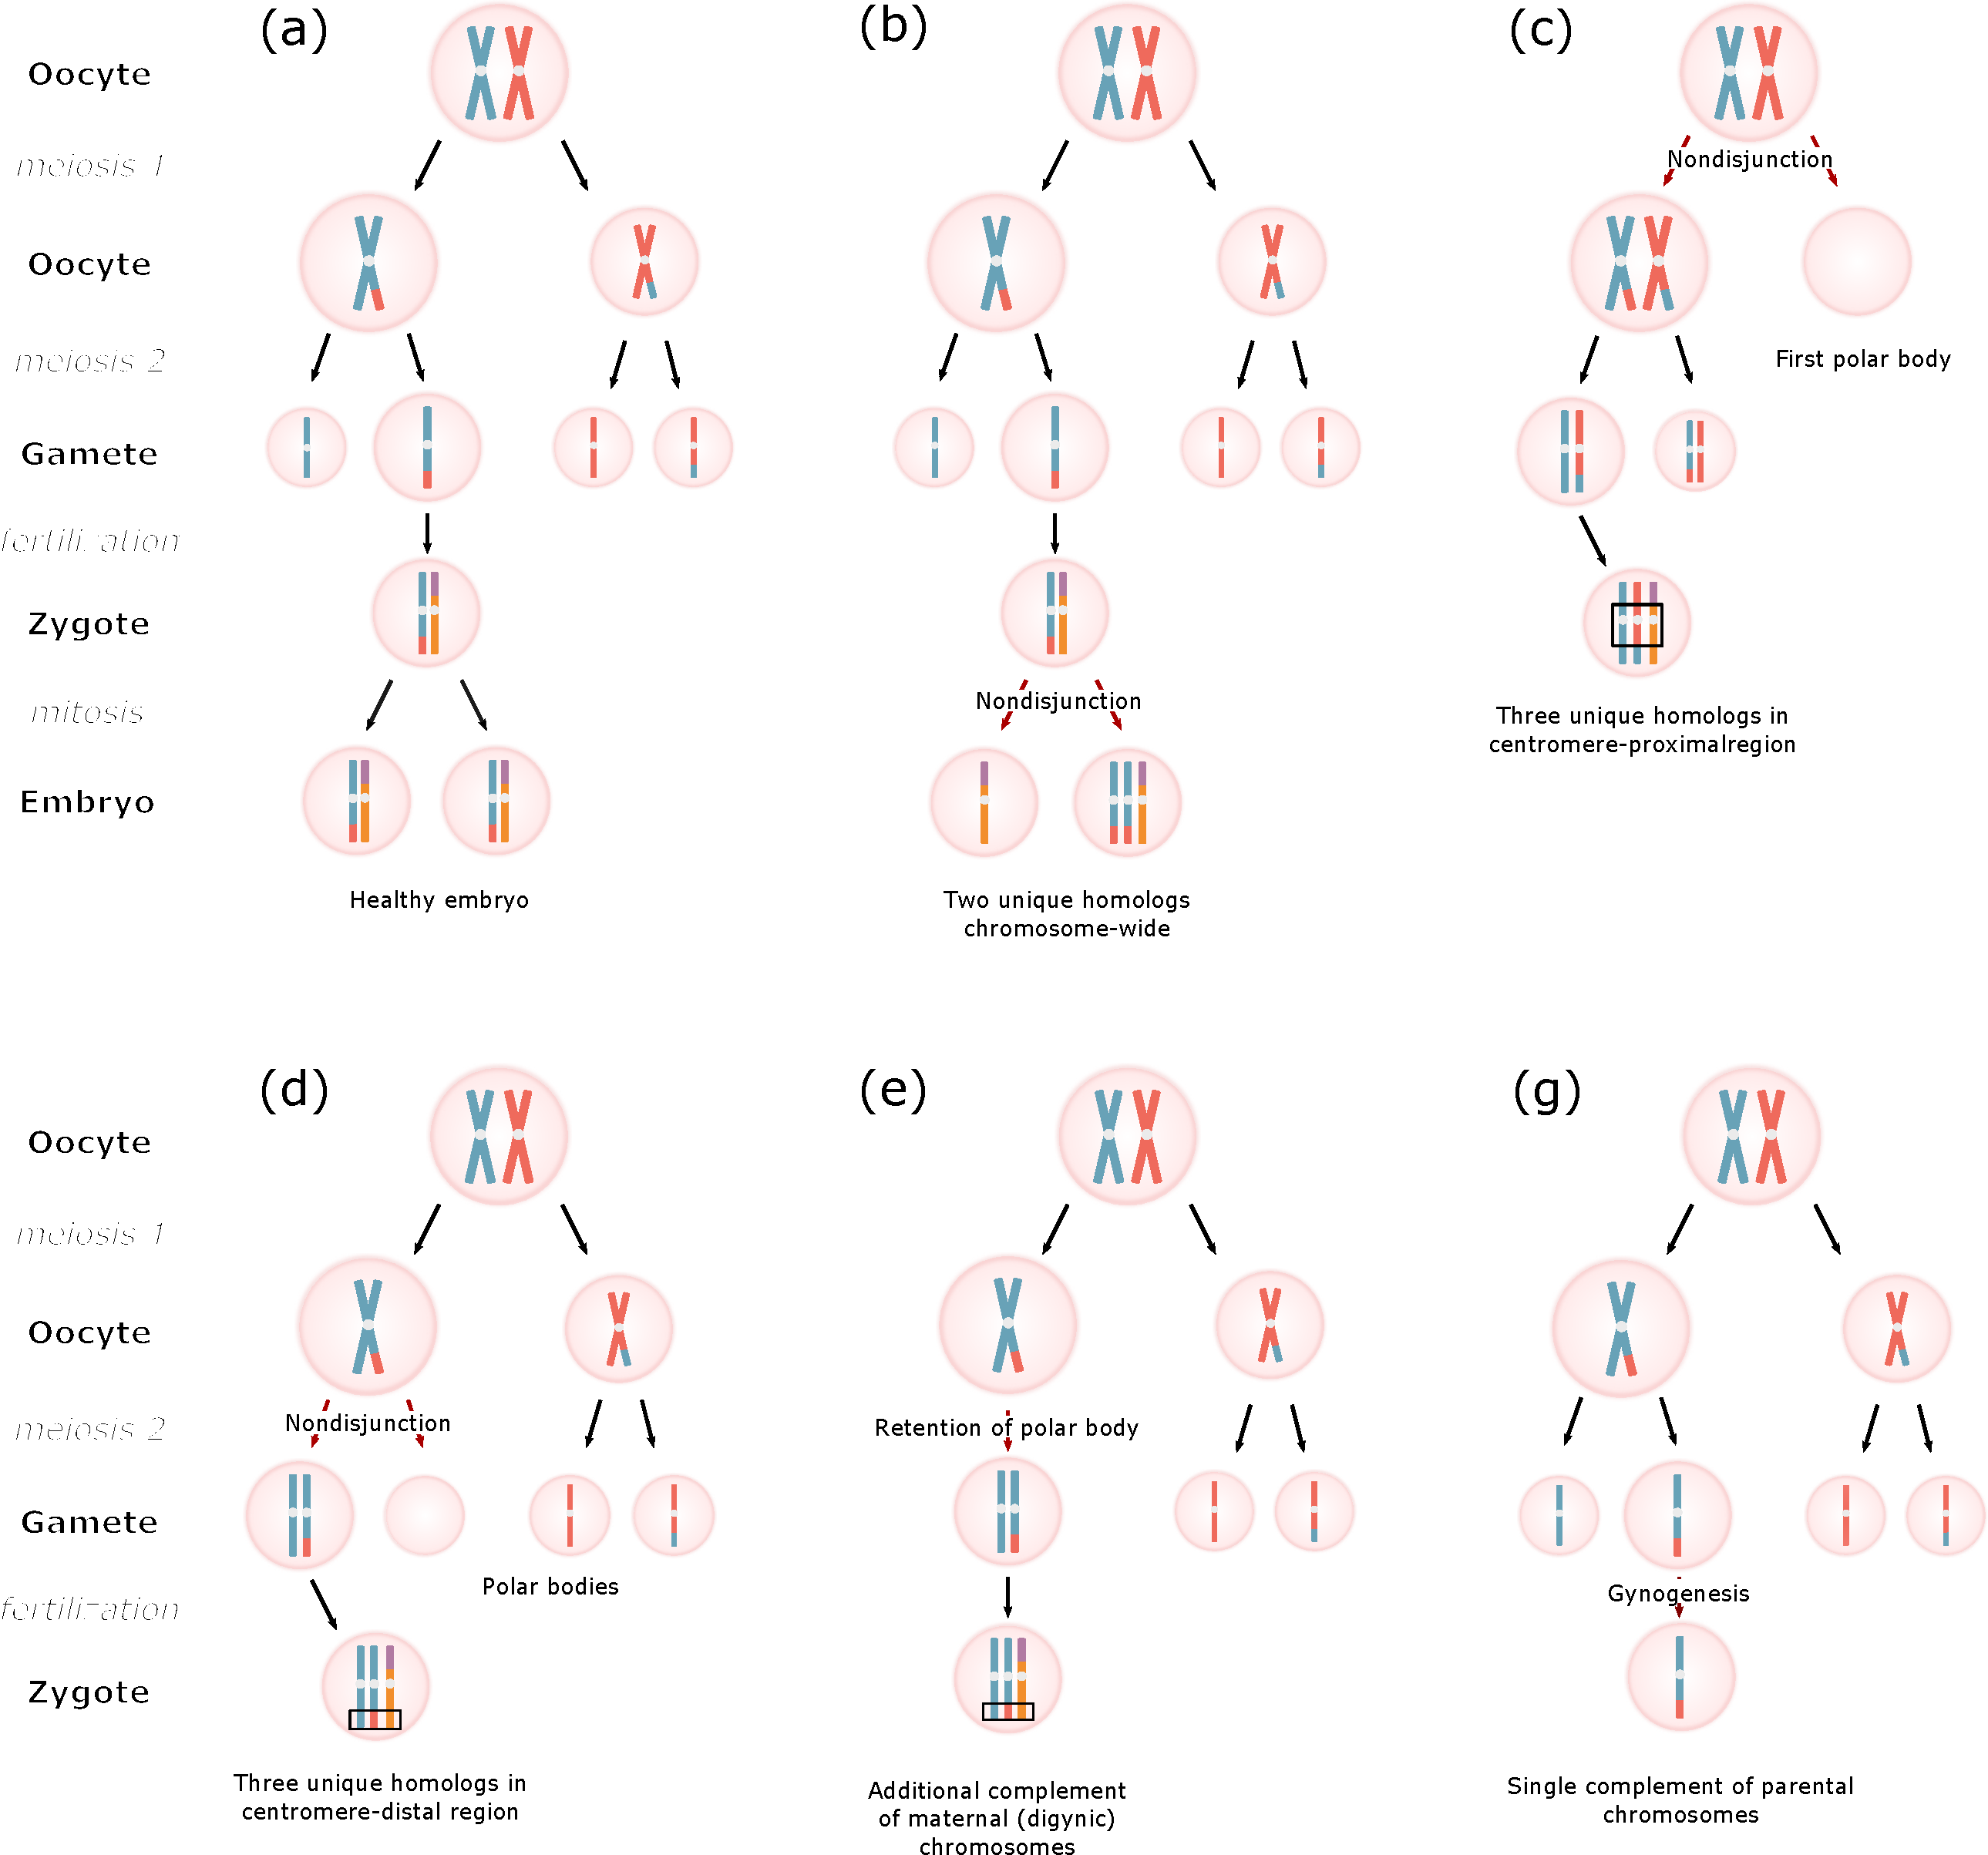
\includegraphics[width=.875\linewidth]{figures/tree5.pdf}

      \caption{Signatures of various forms of chromosome abnormality with respect to their composition of identical and distinct parental homologs. Normal gametogenesis produces two genetically distinct copies of each chromosome---one copy from each parent---that comprise mosaics of two homologs possessed by each parent. Meiotic-origin trisomies may be diagnosed by the presence of one or more tracts with three distinct parental homologs (i.e., transmission of both parental homologs [BPH] from a given parent). In contrast, mitotic-origin trisomies are expected to exhibit only two genetically distinct parental homologs chromosome-wide (i.e. duplication of a single parental homolog [SPH] from a given parent). Triploidy and haploidy will mirror patterns observed for individual meiotic trisomies and monosomies, respectively, but across all 23 chromosome pairs---a pattern that confounds standard coverage-based analysis of PGT-A data.}
    \end{figure}
    
    %\begin{itemize}
    %\item We developed a statistical approach to classify the origins of %trisomies from low-coverage sequencing data. 
    %\item We applied this method to large PGT-A datasets to quantify the %frequencies of errors in meiosis I, meiosis II, and mitosis.
    %
    %\end{itemize}
  \end{block}

  \begin{block}{Classification approach}
      Inspired by the related challenge of imputation, our method overcomes the sparse nature of the data by leveraging haplotype structure from a population reference panel. 
  \begin{figure}
      \centering
     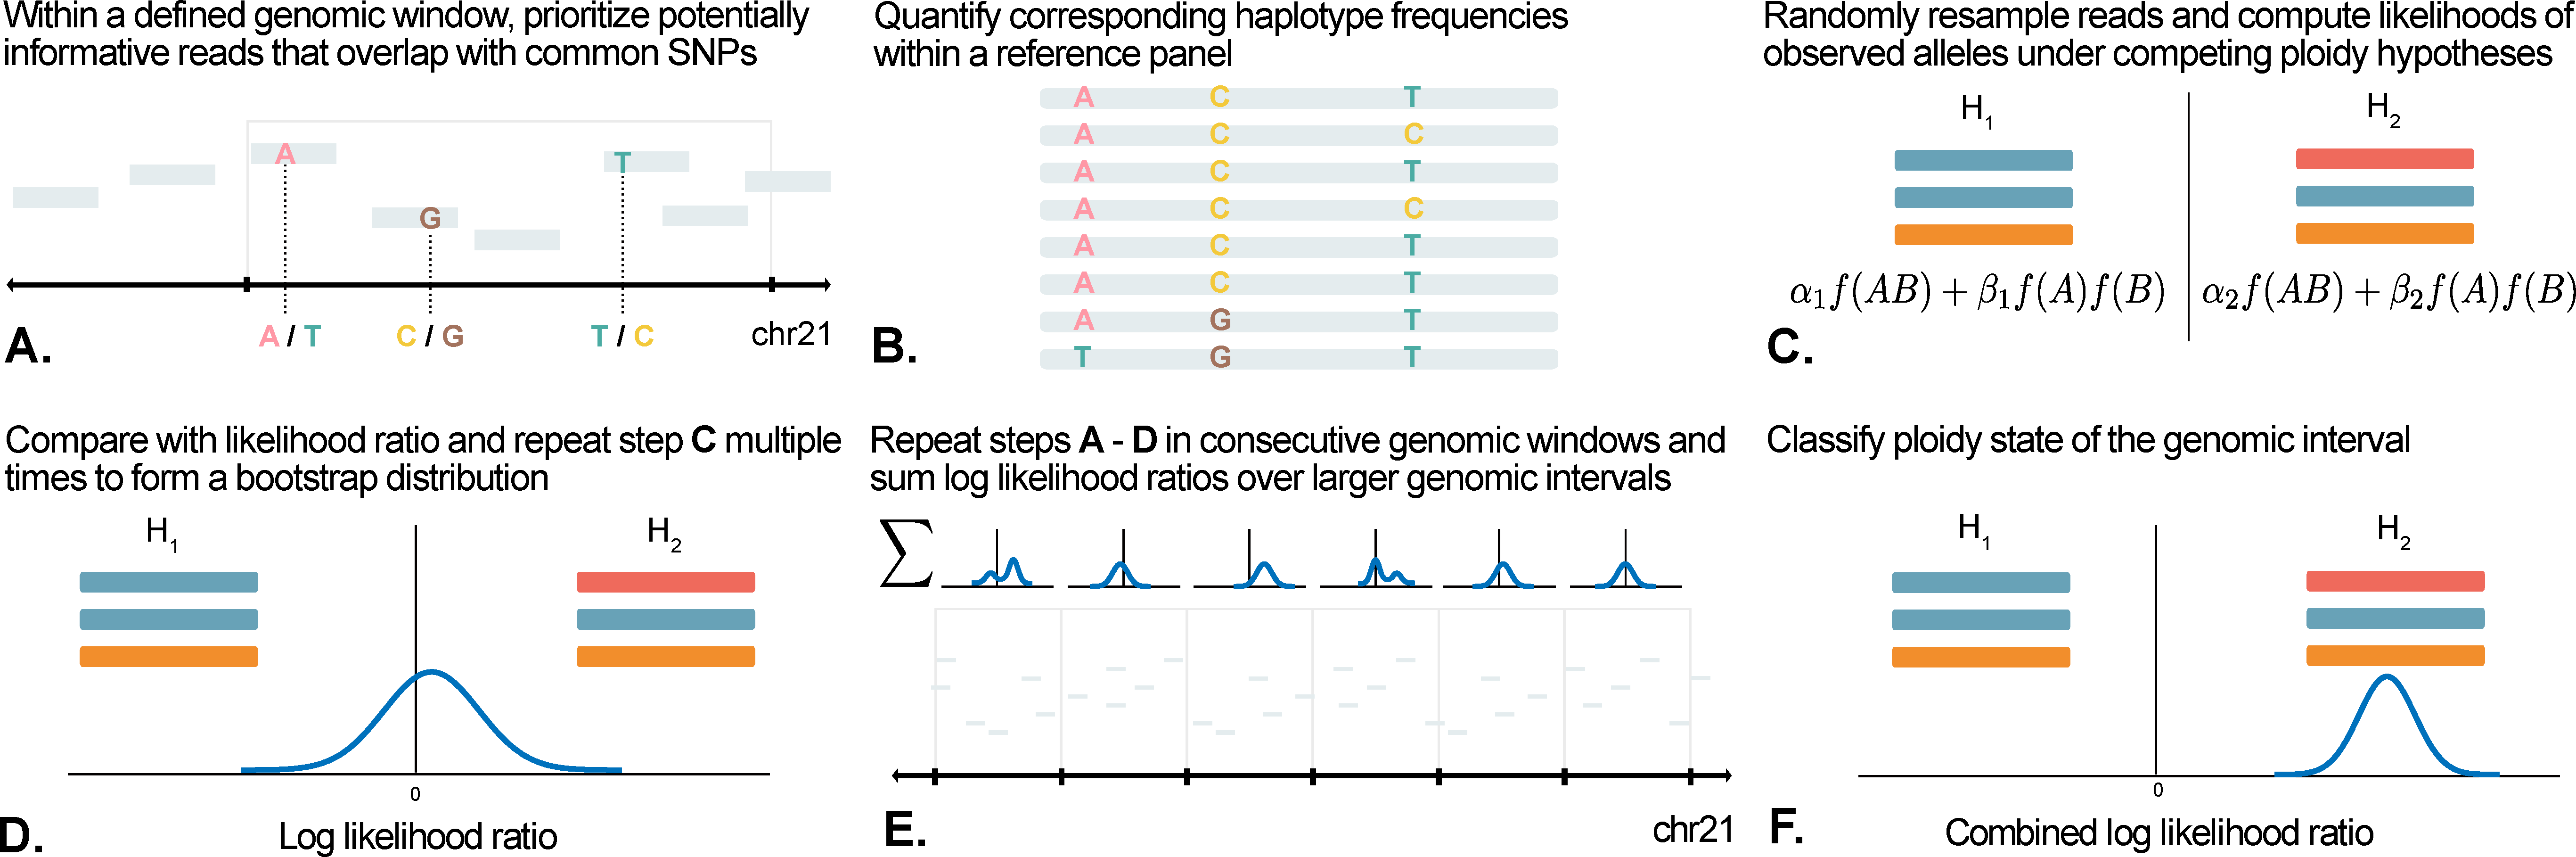
\includegraphics[width=\linewidth]{figures/fig2.pdf}

      \caption{A statistical approach to leverage aneuploidy signatures to classify meiotic and mitotic trisomies using low-coverage sequencing-based data. }
    \end{figure}
    %\begin{itemize}
         
    %\item Scanning across windows of the genome, we compute the probabilities of the observed combinations of alleles given their frequencies and patterns of linkage disequilibrium (LD) in the reference panel. We then compare these “likelihoods” using a likelihood ratio, aggregating signals across consecutive windows. 
    %\item The method retains power to distinguish meiotic and mitotic trisomies down to coverage as low as 0.05x.
    %At higher coverage can also distinguish between meiosis I and meiosis II errors based on signatures flanking the centromeres. 
    %\end{itemize}
  \end{block}
  
\end{column}

\separatorcolumn


\begin{column}{\colwidth}

\begin{block}{Benchmarking with simulation}
\begin{figure}

  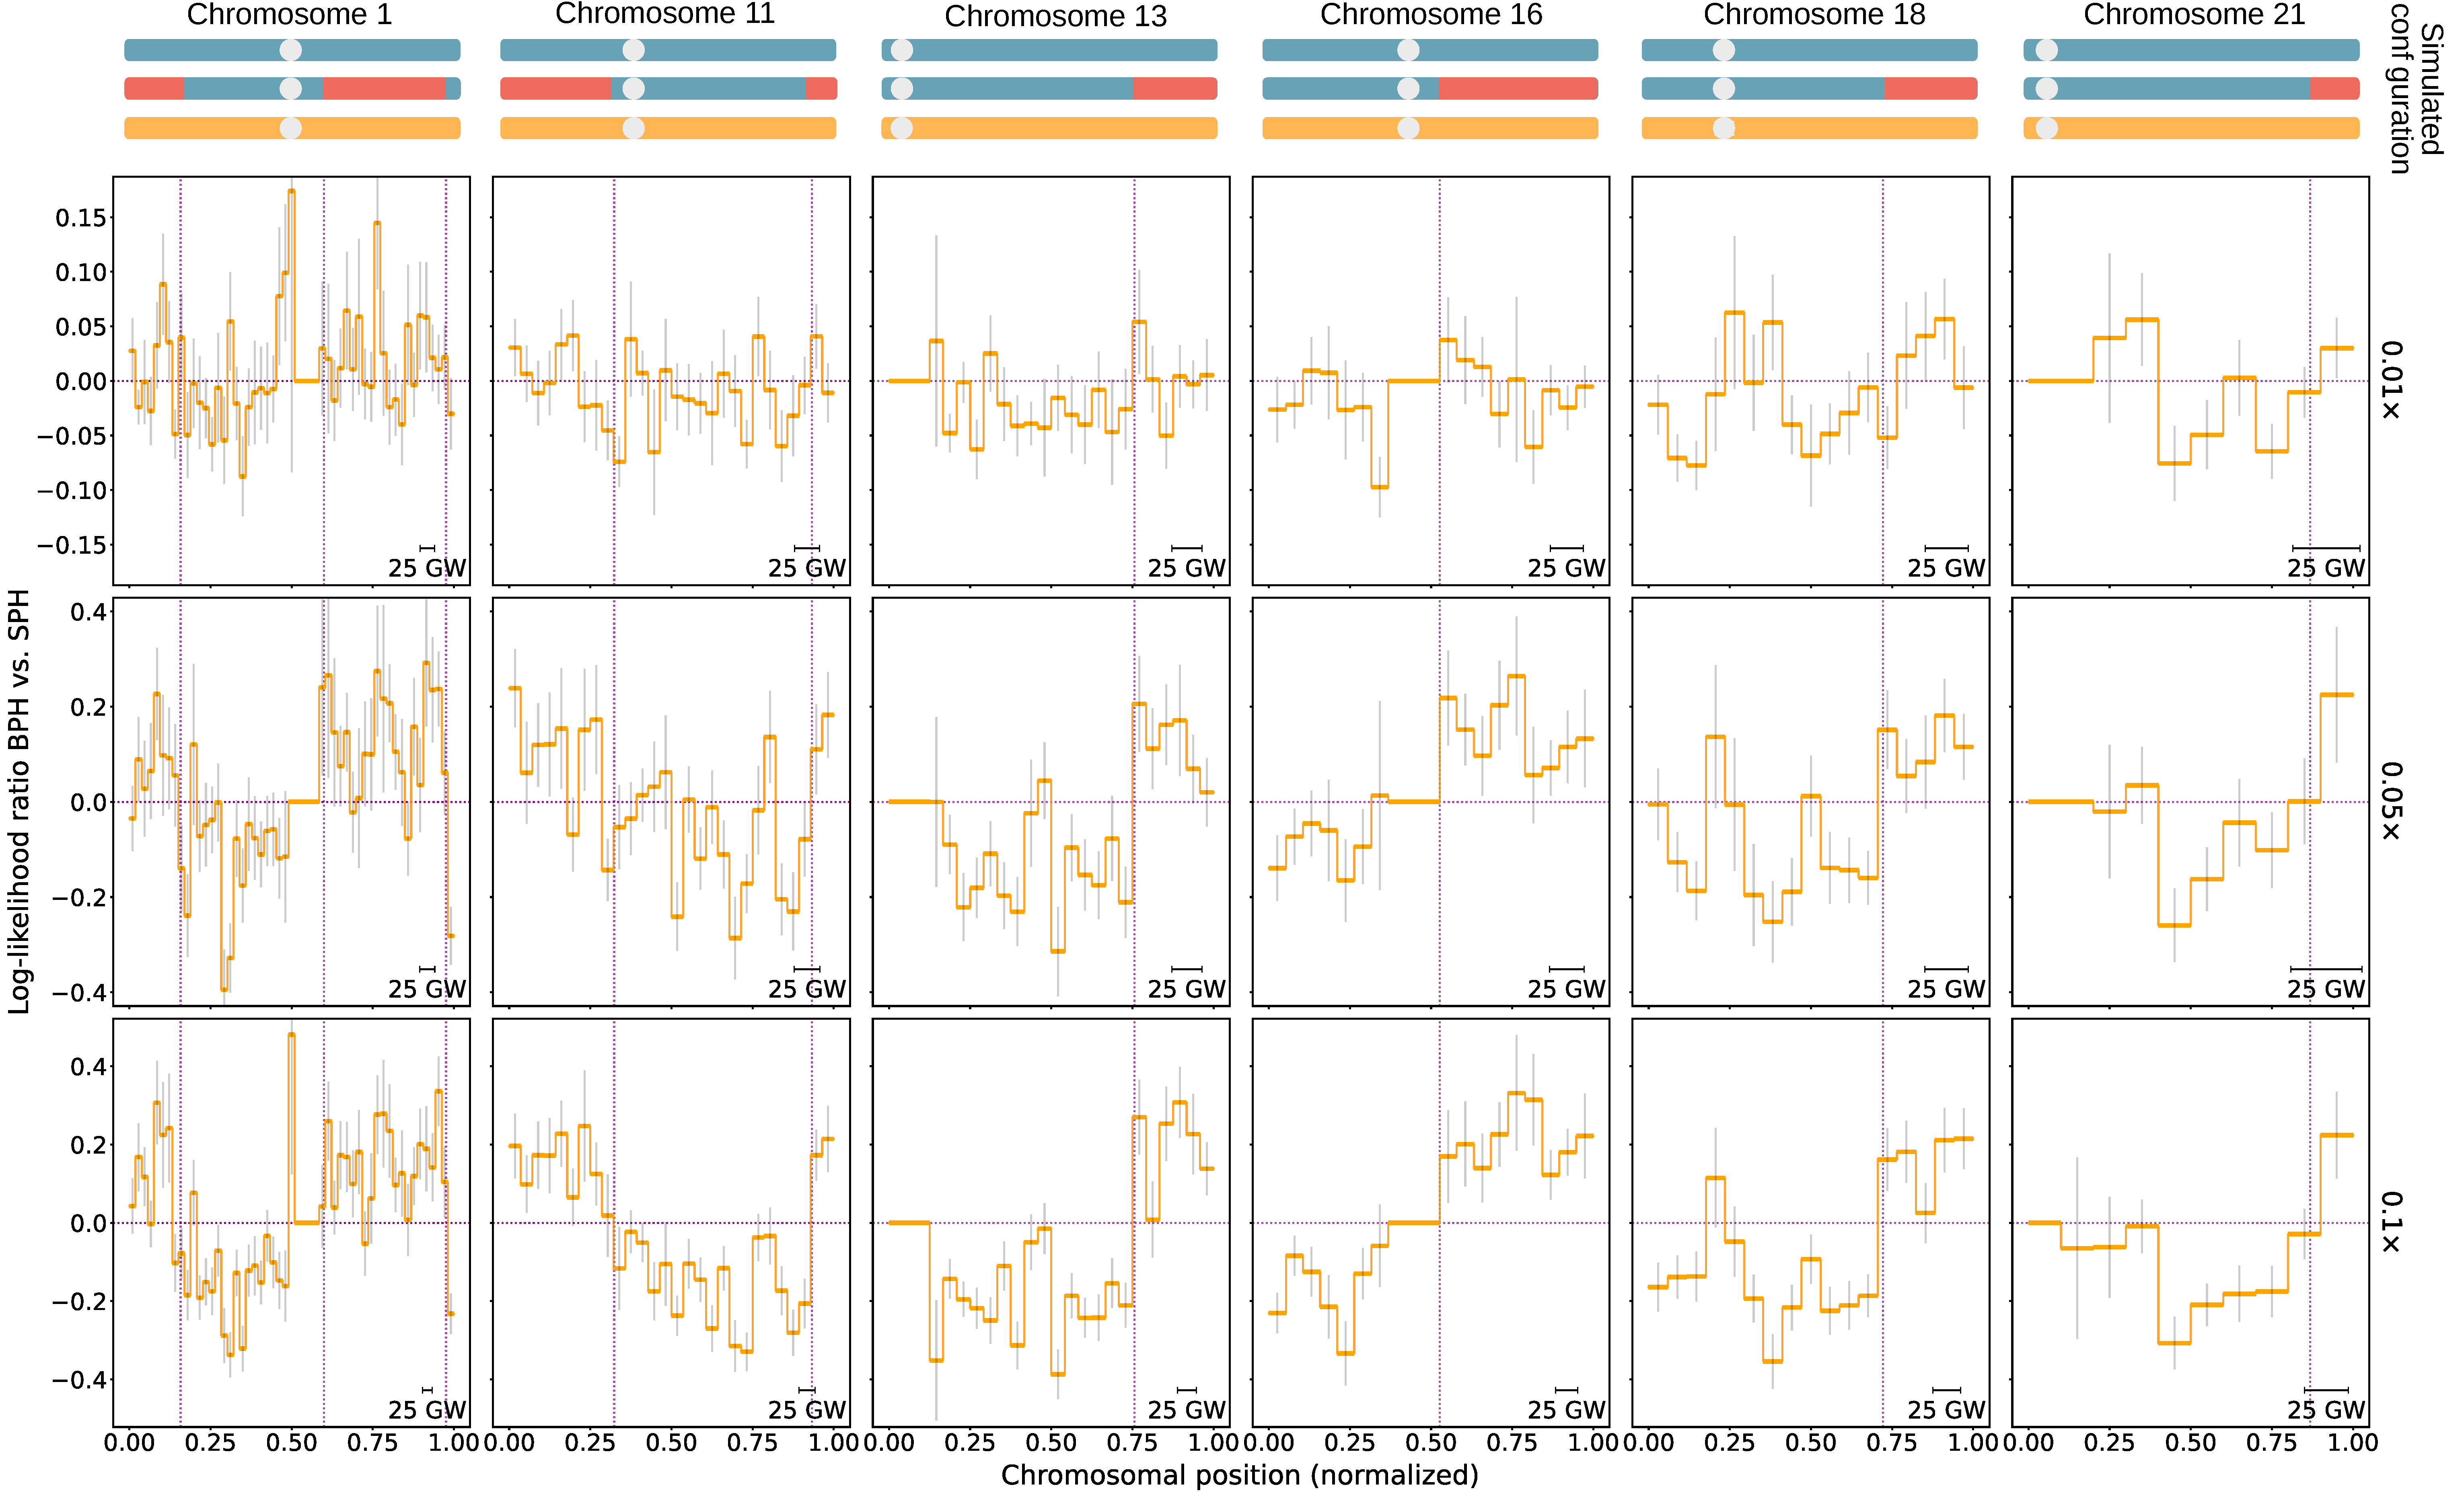
\includegraphics[width=.8\linewidth,align=t]{figures/fig3.pdf}
\caption{Demonstration of the detection of meiotic crossovers.}
 \end{figure}
%\end{block}

%\begin{block}{Balanced ROC curves to benchmark LD-PGTA}
\begin{figure}
\centering
\begin{tabular}{ccc}

  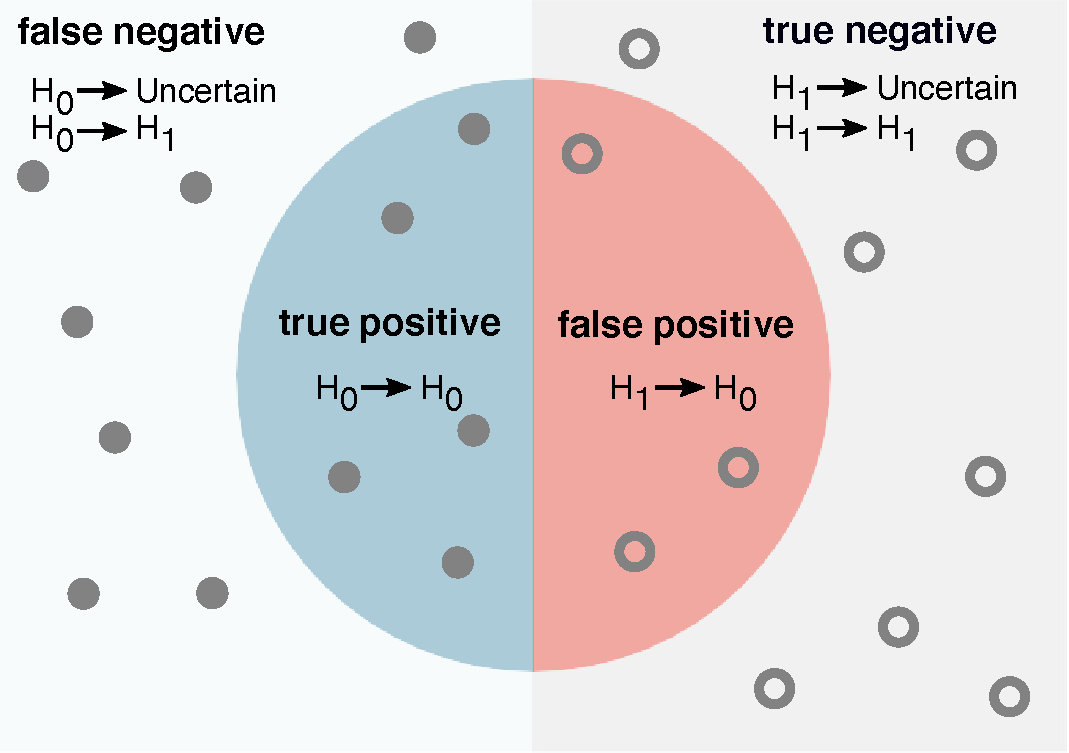
\includegraphics[width=0.27\linewidth,align=c]{figures/fig4a.pdf} &

  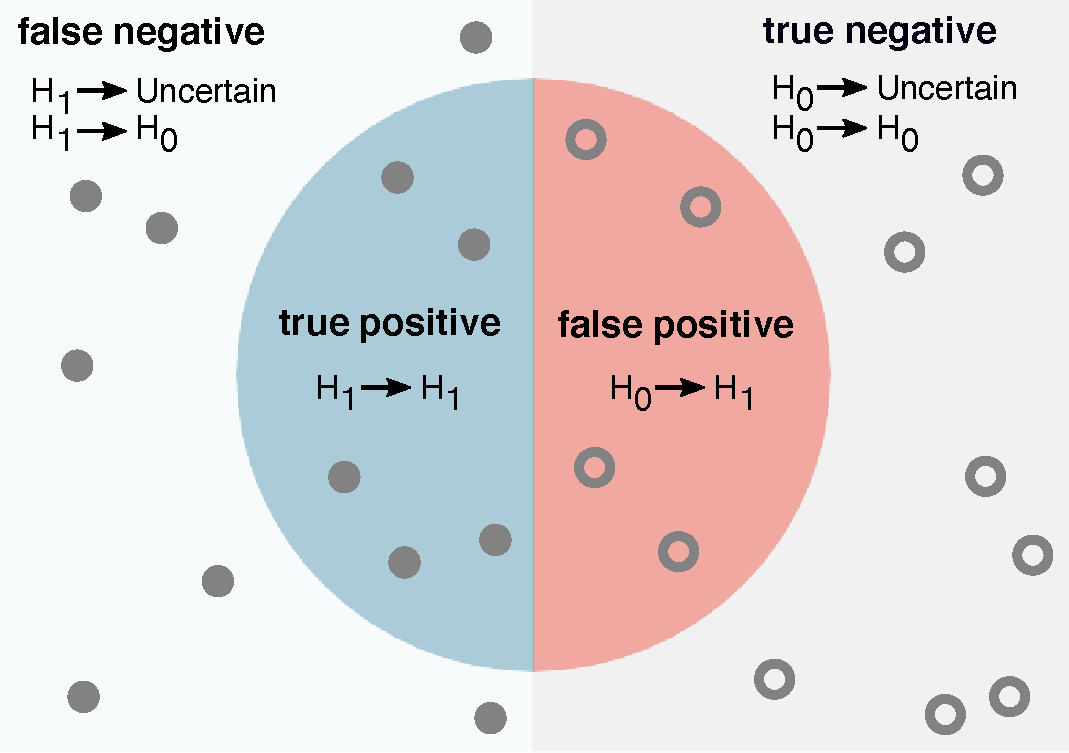
\includegraphics[width=0.27\linewidth,align=c]{figures/fig4b.pdf} &
 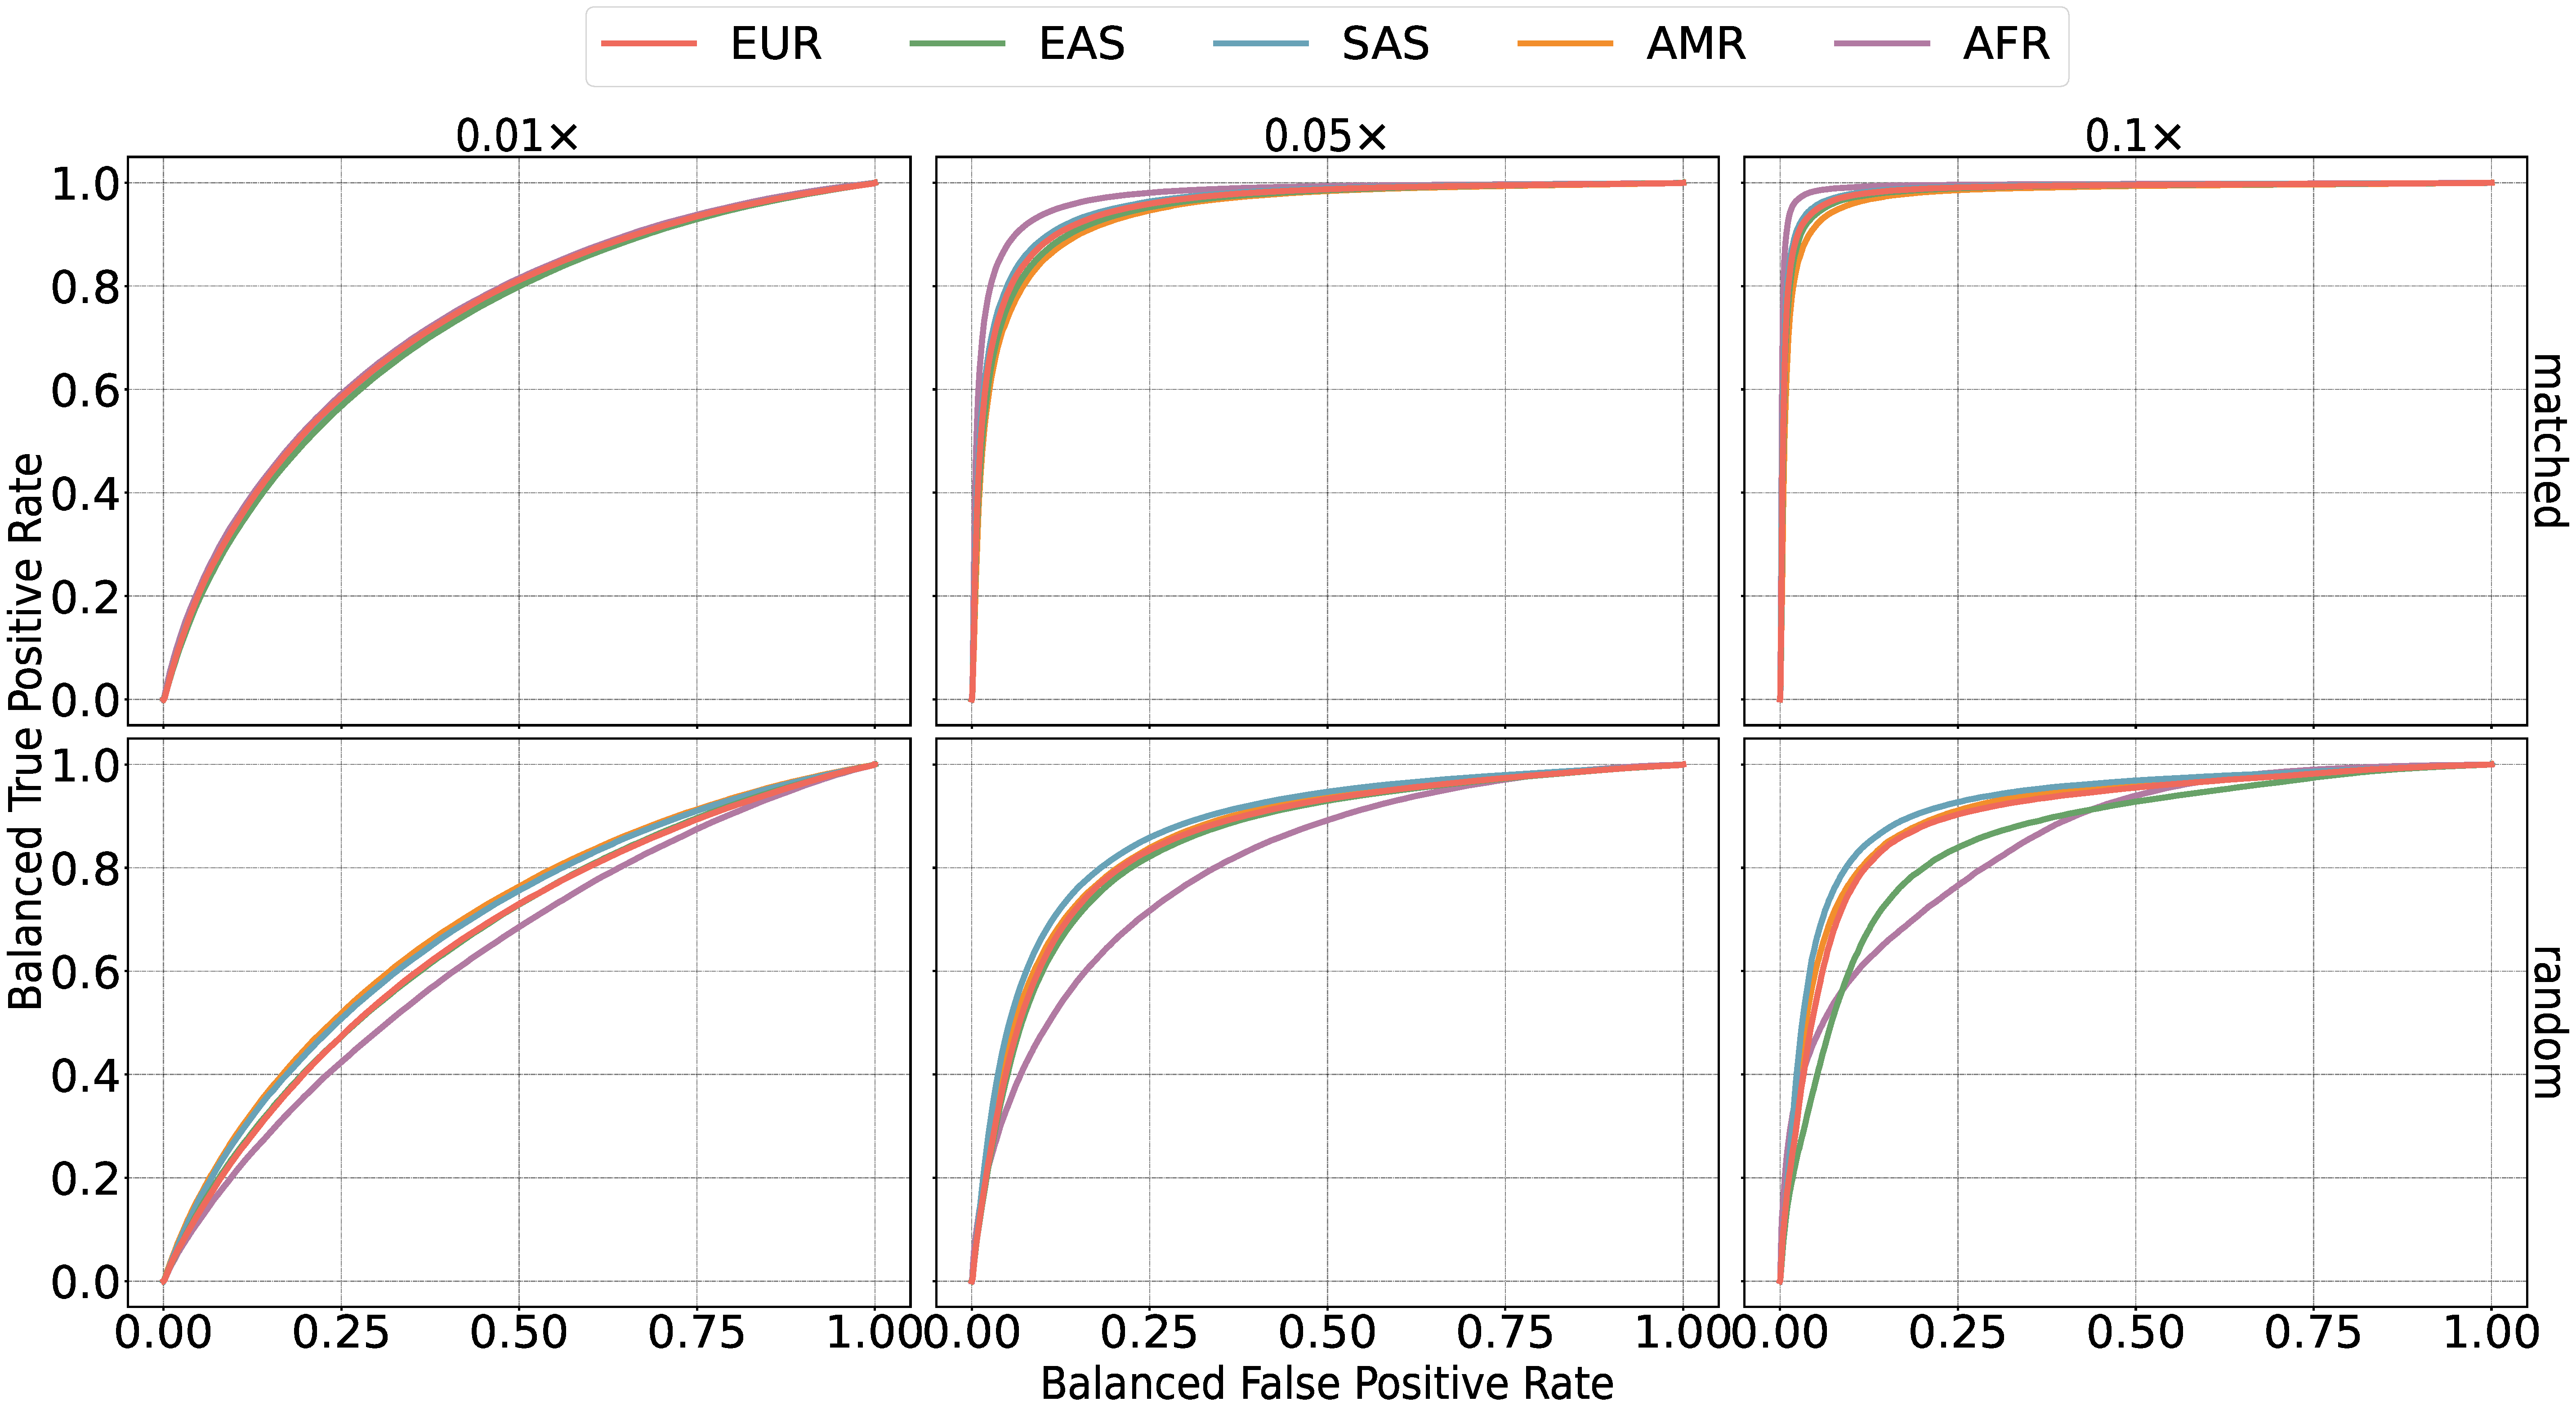
\includegraphics[width=.45\linewidth,align=c]{figures/fig4c.pdf} \\
 \textbf{(a)} & \textbf{(b)} & \textbf{(c)}
  \end{tabular}
  \caption{Balanced ROC curves for BPH vs. SPH with matched and random reference panels of non-admixed embryos, varying depths of coverage. }
 \end{figure}
\end{block}

  \begin{block}{Application to PGT-A data}
  
 We applied our method to low-coverage PGT-A data from $>$8,000 human embryos provided by the Zouves Fertility Center. 
%    \item We will quantify the proportion of IVF cases with no euploid embryos but at least one putative mitotic-origin trisomy that may be considered for transfer.
%\end{itemize}

     \begin{figure}
      \centering
     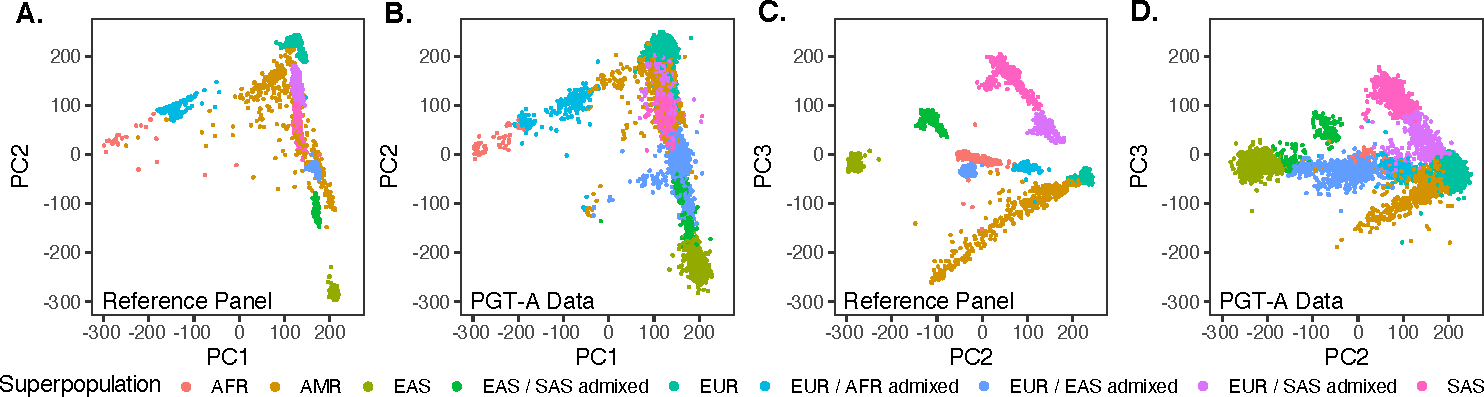
\includegraphics[width=\linewidth]{figures/fig5.pdf}
\caption{Ancestry inference from low-coverage PGT-A data informs the selection of matched reference panels. PCAs were defined based on analysis of 1000 Genomes reference samples. }
\end{figure}
\begin{figure}
     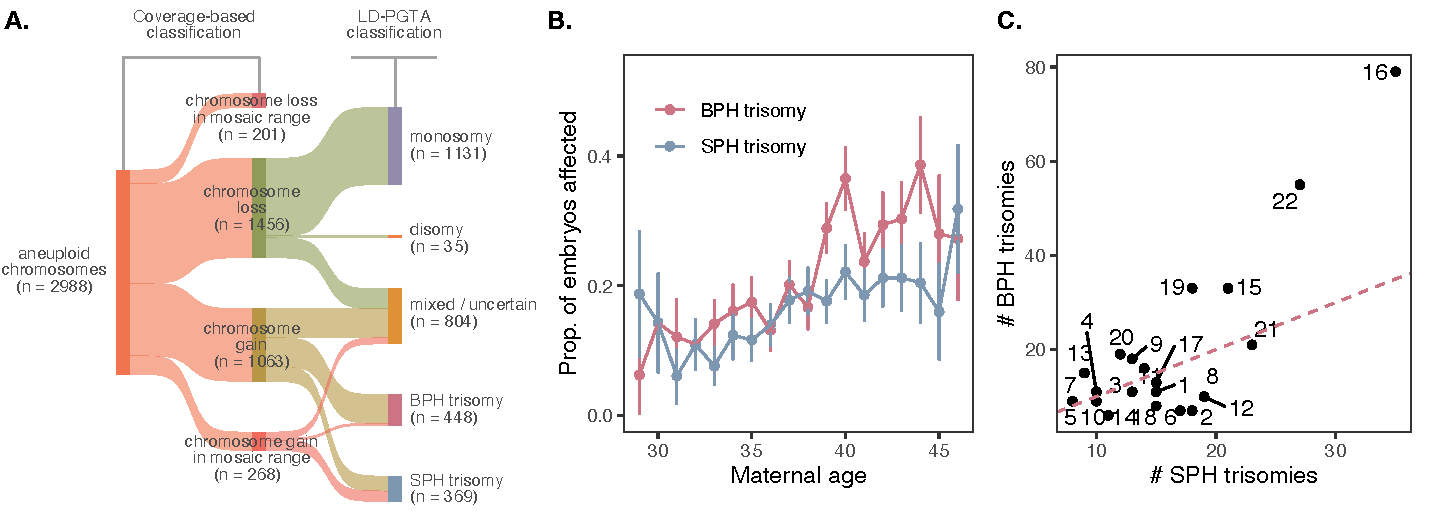
\includegraphics[width=\linewidth]{figures/fig6.pdf}

      \caption{Classification of trisomies of meiotic and mitotic origin (A), their association with maternal age, and their chromosome-specific propensities.}
    \end{figure}
  \end{block}

%    \begin{table}
%      \centering
%      \begin{tabular}{l r r c}
%        \toprule
%        \textbf{First column} & \textbf{Second column} & \textbf{Third column} & \textbf{Fourth} \\
%        \midrule
%        Foo & 13.37 & 384,394 & $\alpha$ \\
%        Bar & 2.17 & 1,392 & $\beta$ \\
%        Baz & 3.14 & 83,742 & $\delta$ \\
%        Qux & 7.59 & 974 & $\gamma$ \\
%        \bottomrule
%      \end{tabular}
%      \caption{A table caption.}
%    \end{table}


\end{column}

\separatorcolumn
\begin{column}{\colwidth}


\begin{block}{Revealing abnormalities in genome-wide ploidy}
    
    \begin{figure}
      \centering
     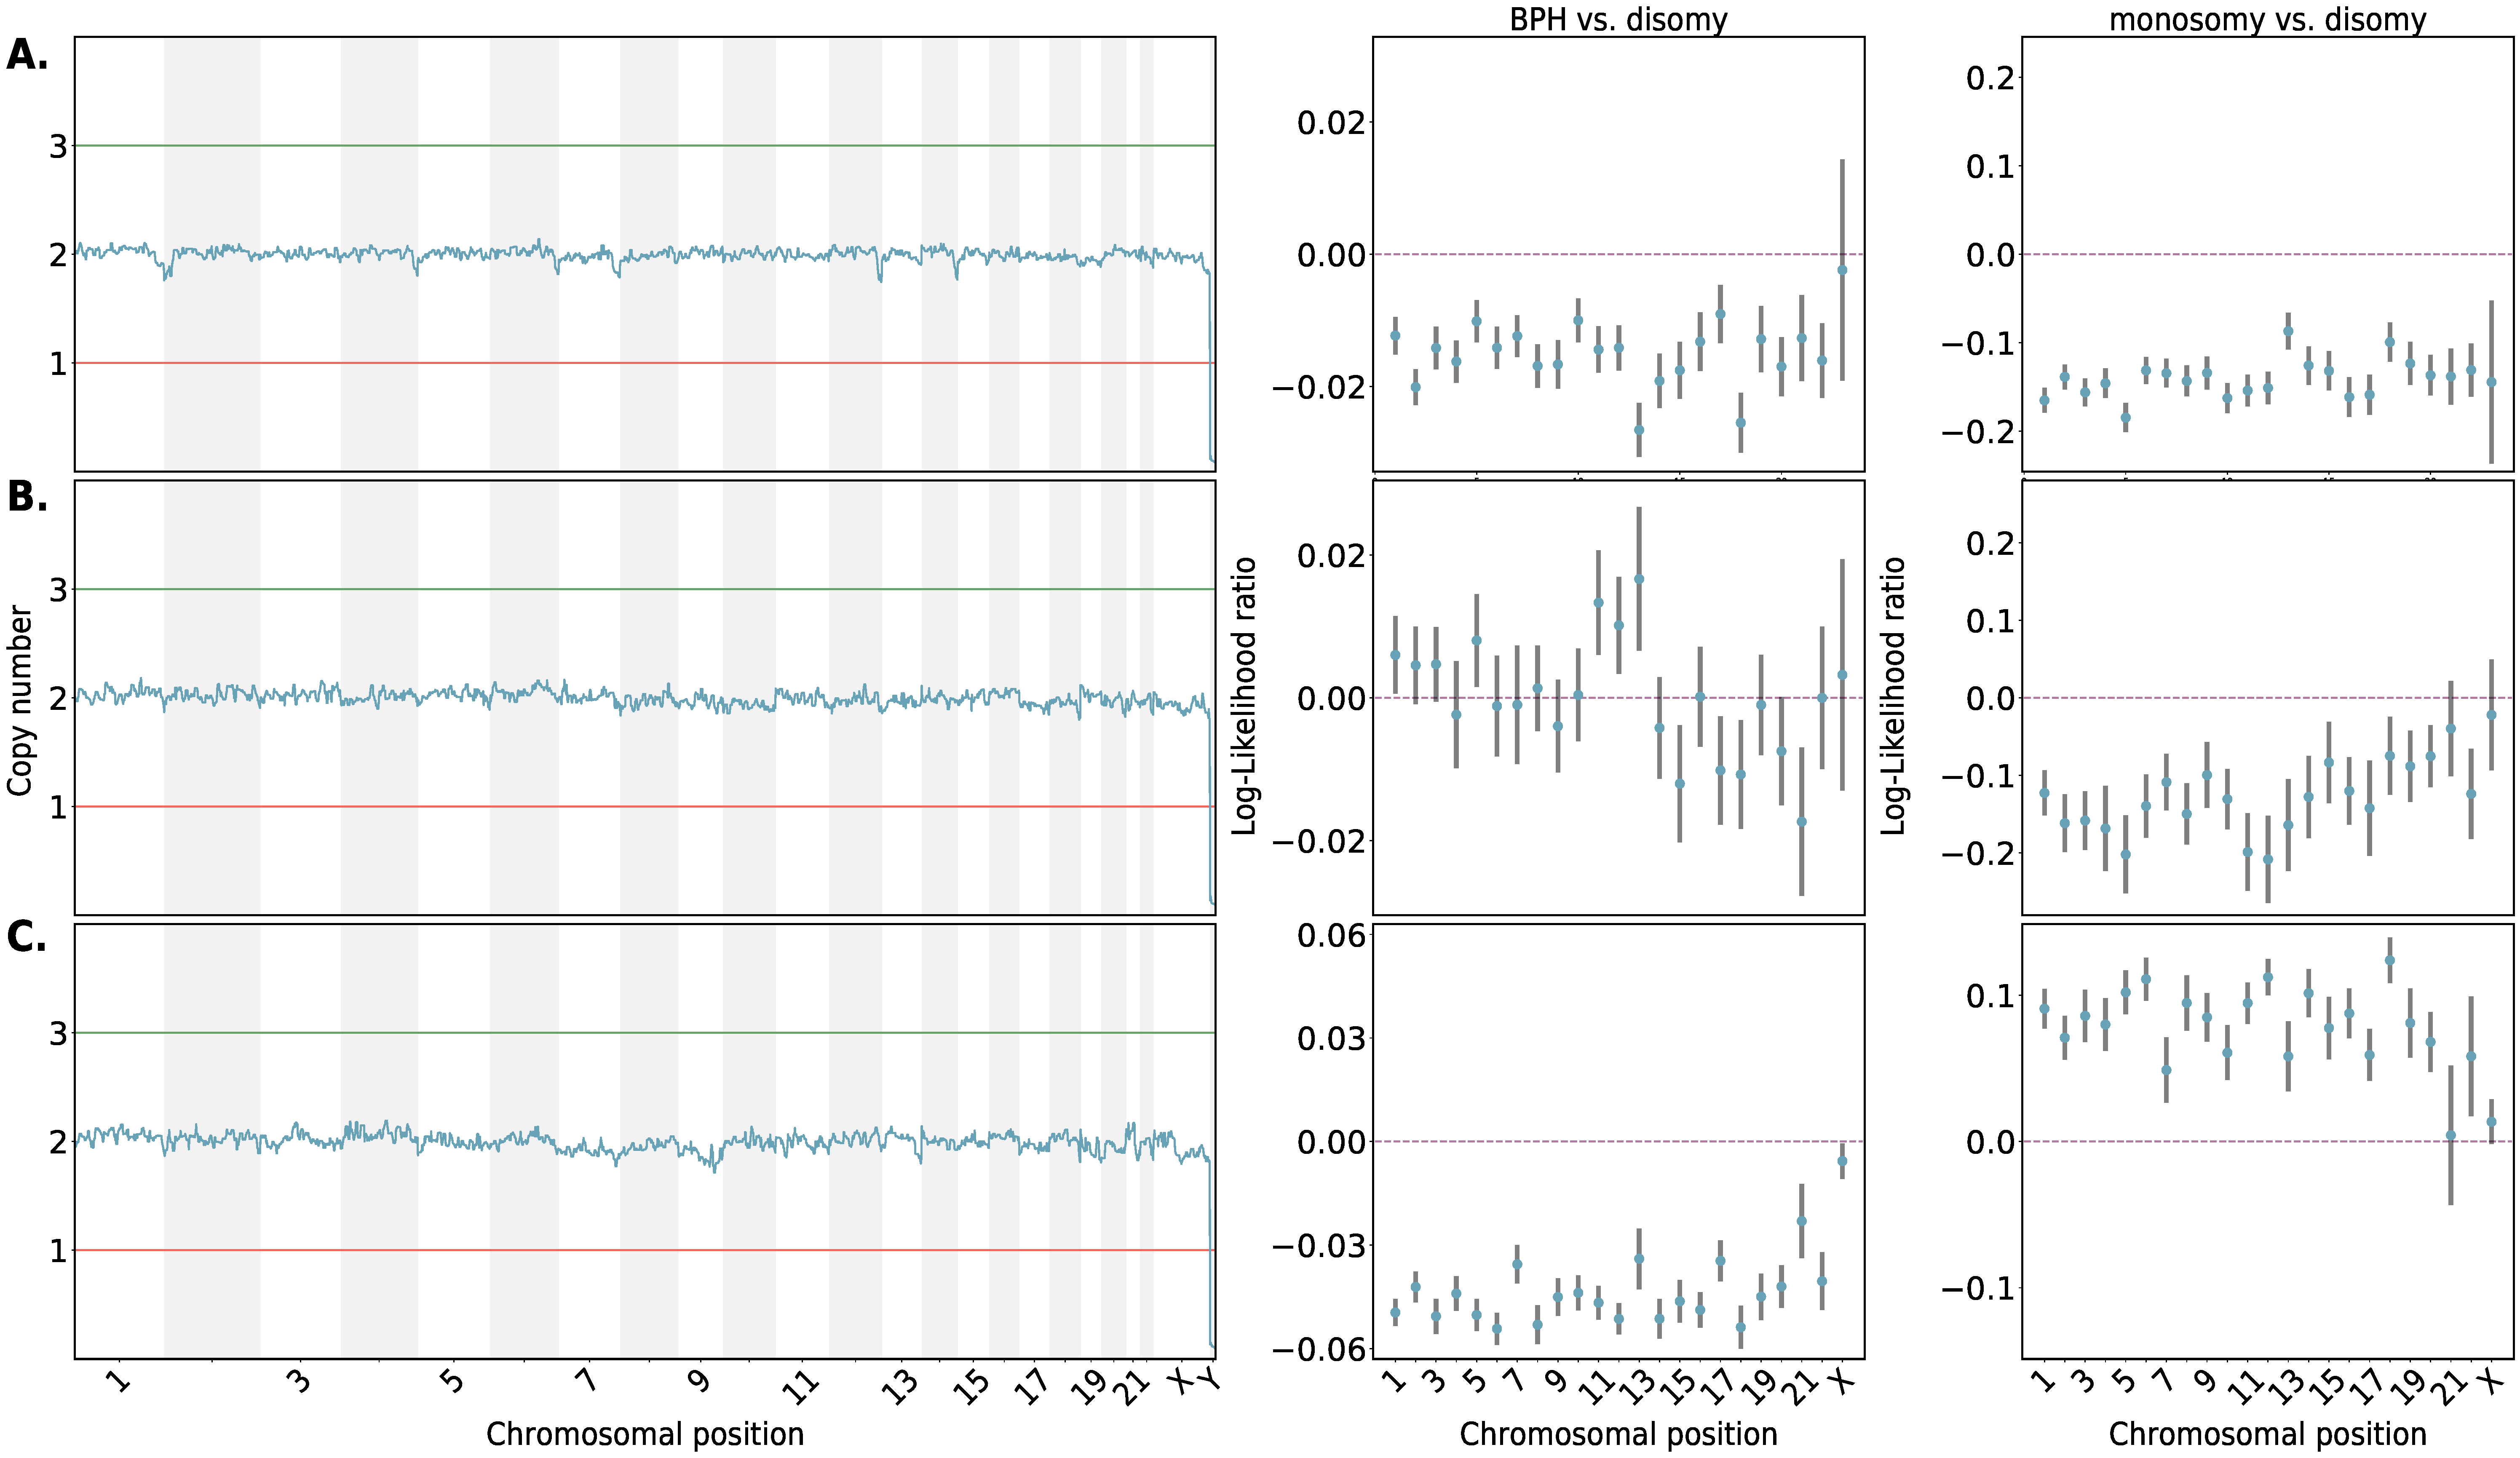
\includegraphics[width=.8\linewidth]{figures/fig7.pdf}

      \caption{Representative putative diploid (A.), triploidy (B.), and haploid (C.) samples.}
    \end{figure}
\end{block}

\begin{block}{Mapping meiotic crossovers}

        \begin{figure}
      \centering
     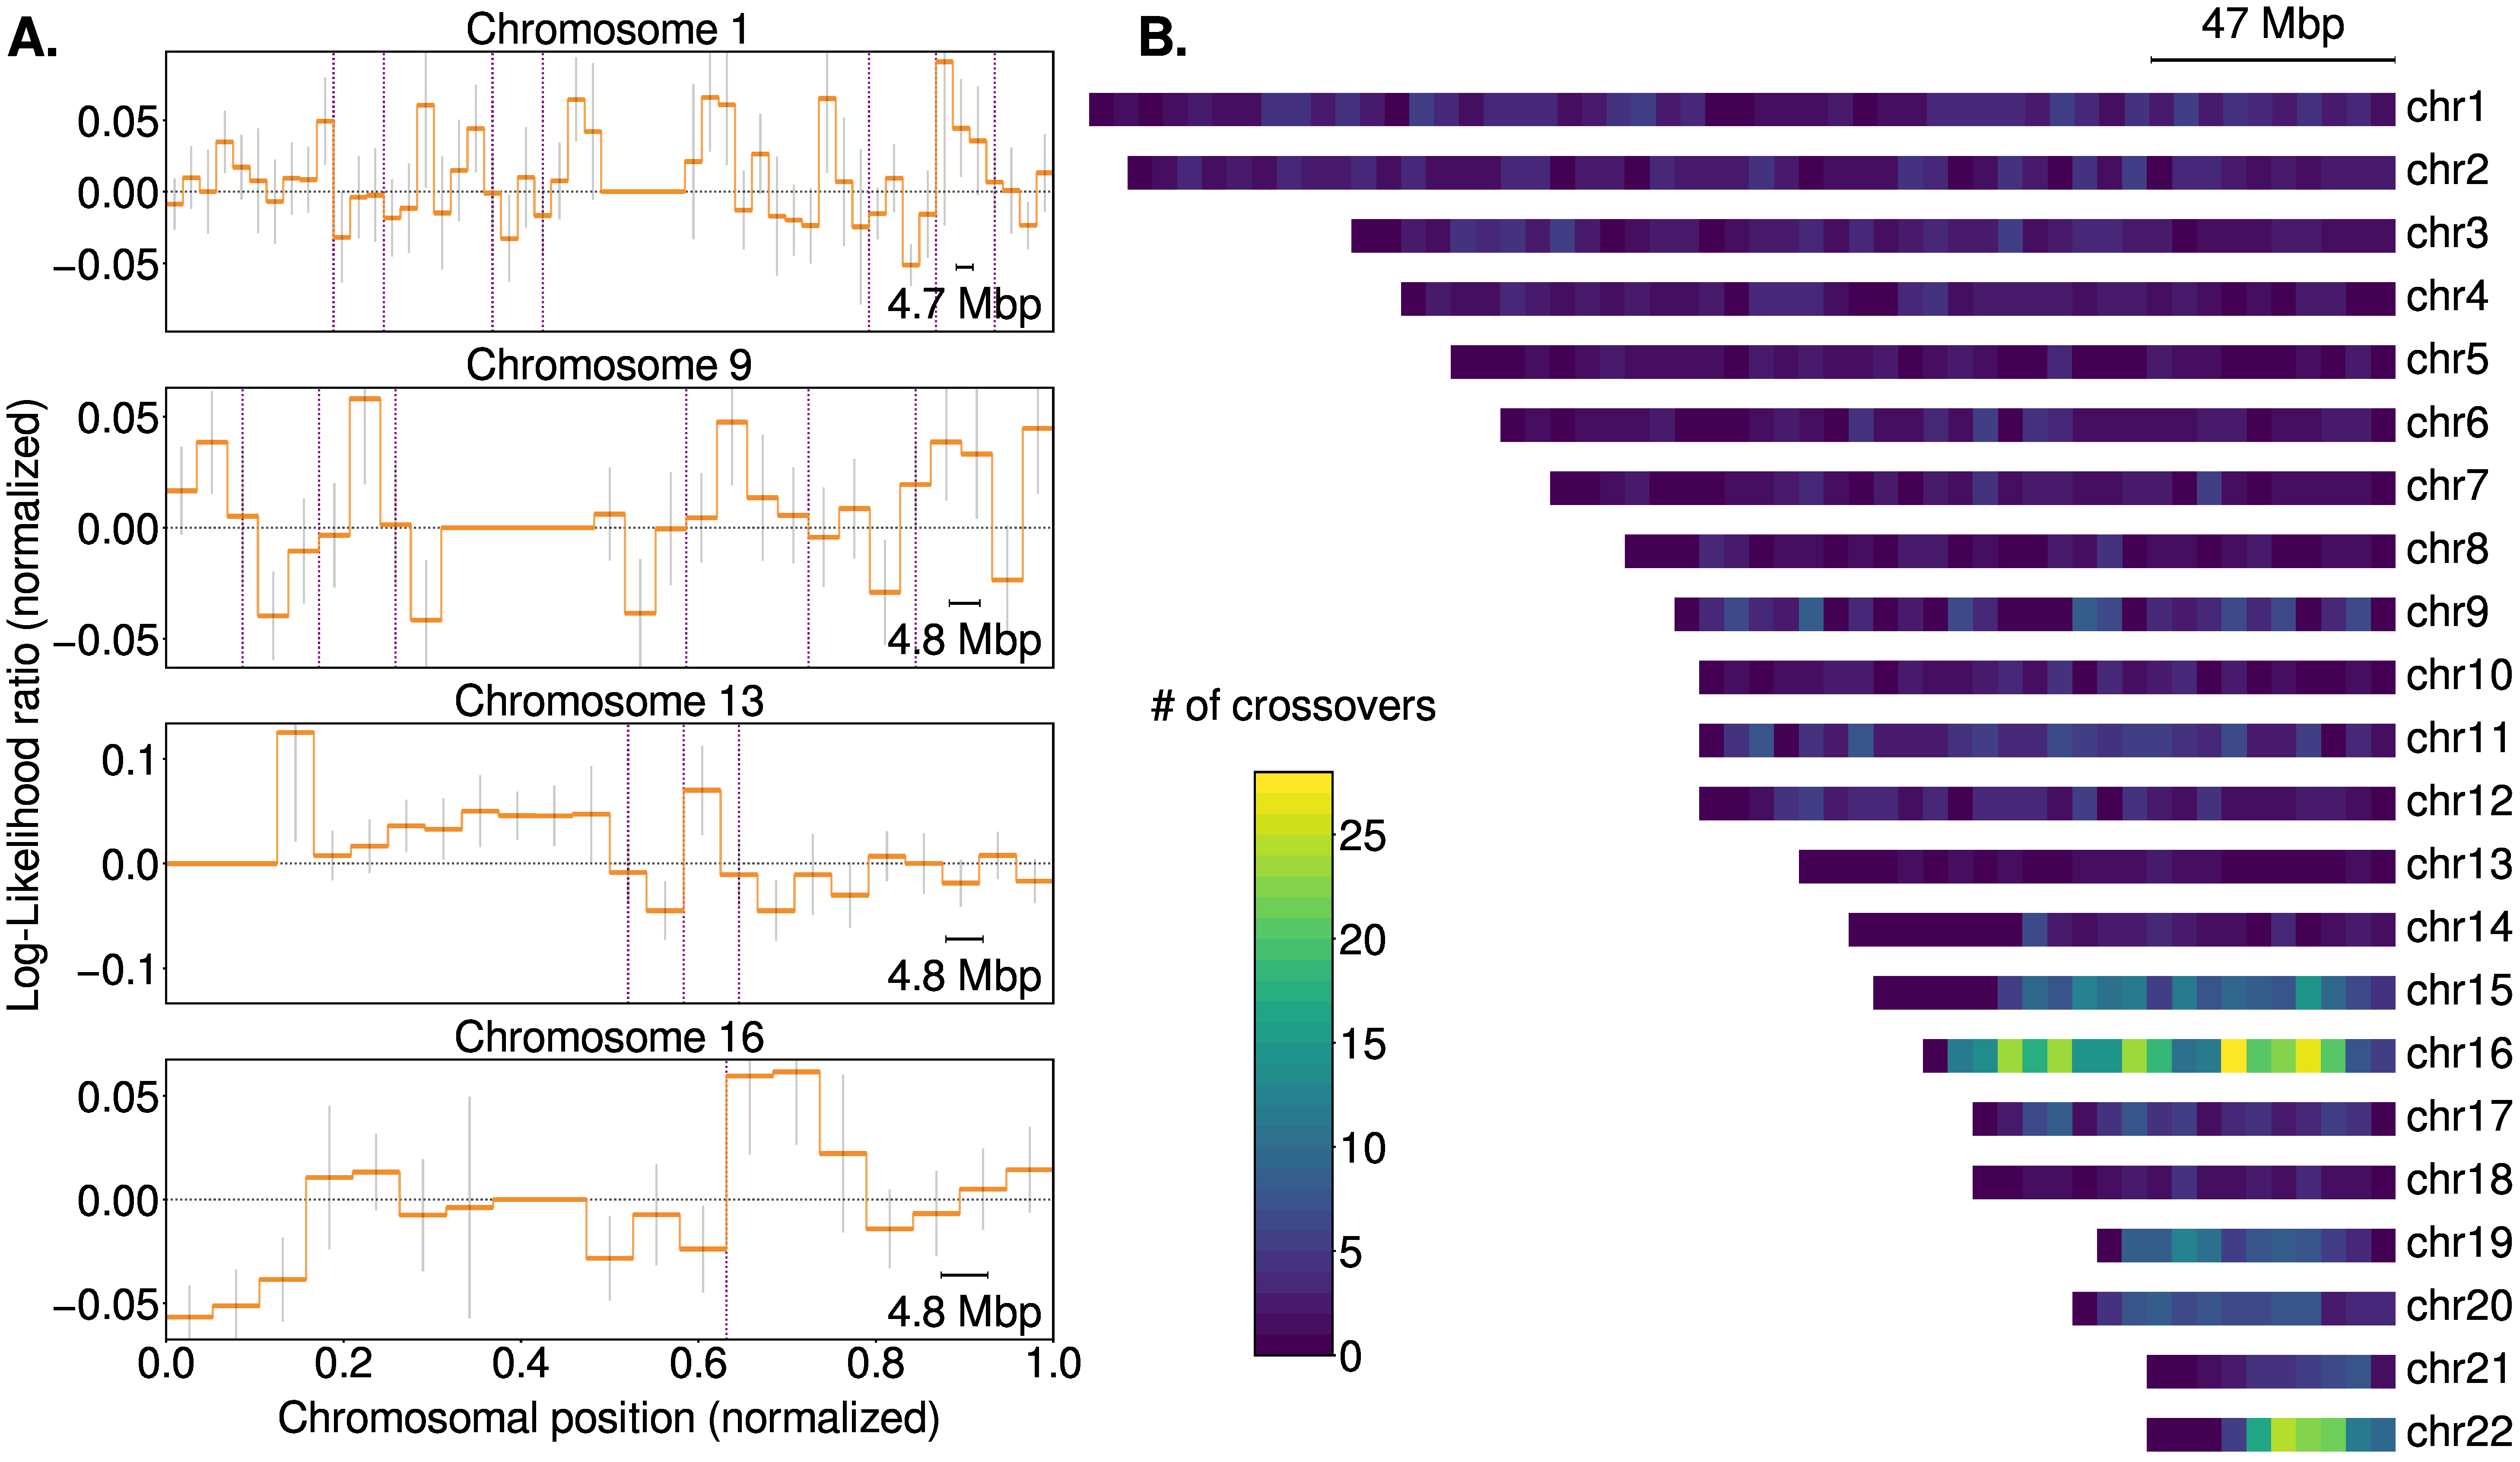
\includegraphics[width=.8\linewidth]{figures/fig8.pdf}

     \caption{Mapping of meiotic crossovers on putative trisomic chromosomes based on inferred switches between tracts of BPH and SPH trisomy.}
    \end{figure}
\end{block}
    
\begin{block}{Conclusions}
\begin{itemize}
	\item{Aneuploidies arising during 
	meiosis and mitosis have distinct impacts on development and possess unique haplotype signatures.}
	\item{We distinguish these signatures from low-coverage sequencing.}
    \item{Potential to improve IVF outcomes and diagnosis of pregnancy loss.}
\end{itemize}
\end{block}

\begin{block}{Acknowledgements}\footnotesize
Research reported in this poster was supported by National Institute of General Medical Sciences of the National Institutes of Health under award number R35GM133747.
\end{block}

  \begin{block}{References}

    \nocite{*}
    \footnotesize{\bibliographystyle{siam}\bibliography{poster}}

  \end{block}
\end{column}
\separatorcolumn

\end{columns}
\end{frame}

\end{document}
